\chapter{Results and Discussion}

This purpose of this chapter is to describe the testing prodecures, results, and implementation issues that were encountered during the implementation phase of the project. Whenever possible, concrete results will be compared with those described previously in Ch.\ \ref{cha:goals}. The amount of work accomplished with each module will also be discussed.

The Engine and Transmission, and Braking modules both require that the Formula SAE 2010 vehicle be at least partly complete for testing. Since the build schedule for the vehicle is to have it complete for the beginning of May, 2010, much of the final-stage testing and tuning of these modules was not yet possible as of writing. Additionally, a prototype of the full pneumatics system was not ready for writing.

\section{Transmission}

\subsection{Electro-pneumatic Simulation}


\subsection{System testing}

Since testing and tuning of the full electro-pneumatic system requires that the 2010 Formula SAE vehicle be complete, this phase of the project was not completed as intended, and is recommended for future work.

\section{Intake}

As of writing, the Formula SAE team members responsible for designing and implementing the two stage intake-plenum were still in the design stages of that project. Our contributions to the variable intake-plenum project, namely the electronics to provide the control signal from the engine and transmission module, are complete. Completing the control software and testing this system will need to be done after the intake is fully designed and manufactured.

\section{Braking}

\begin{figure}[htp]
 \centering
 \includegraphics[width=5in,keepaspectratio]{results/figures/brake_module_test_bench.eps}
 \caption{Braking module bench testing.}
 \label{fig:brake_module_bench_test}
\end{figure}


\subsection{Bias Adjustment}


\subsection{Calibration}


\section{Telemetry}

Getting the software implementation of the Telemetry module to work successufully was far more difficult than originally imagined. The individual components of the system software would run as expected on their own, but fail when coupled together. For example, the ECU data link and the DAC data link were at one point in the software development process relatively stable in operation by themselves, but enabling both would cause data loss, or one of the two links to drop. A large amount of time was invested in investigating the causes of these problems, and will be discussed in this section.

\subsubsection{Wireless Data Link}

We had originally planned to run the wireless link's data rate higher than \unit{115,200}{\bit\per\second}. The XBee documentation states that the modem is capable of running up to \unit{250,000}{\bit\per\second}, and the XBee modems allow for a continuous range of baud rates to be selected. Unfortunately it was determined when we started testing the Telemetry module software that the XBee could not in fact set it's baud rate to the highest possible with the MAX3100 was capable of: \unit{230,400}{\bit\per\second}.

The MAX3100 was therefore configured to operate at \unit{115,200}{\bit\per\second}, and the XBee modem's interface rate was matched. A simple throughput stress test was performed that continuously wrote data in 16 byte chunks into the MAX3100's driver's software transmit buffer. A fixed-length 32 byte software buffer was never overrun with this test, and an actual data throughput of $\unit{8.251}{\kilo\byte\per\second}$ was observed with a logic analyser on the TX pin of the MAX3100.

\subsection{Data Interfaces}

\subsubsection{ECU }

\subsubsection{DAC }



\subsection{Interrupt Starvation on the Telemetry Module}

Issues caused by the large degree of asynchronous behaviour in the system, and the large number of common resources used. Multiple producer/consumer layers. Solved by ensuring that atomic sections were placed around critical code.

Although initial average data throughput rates for both the DAC and the ECU were measured as part of the research done at the beginning of the project, non-trivial buffering issues did arise in the implementation of the telemetry module software. After several weeks of work spent debugging throughput problems with the module software, and with the aide of a protocol analyser, the root of the problem was tracked down. The AT90CAN microcontroller's interrupt vectors are fixed at the factory, therefore the priority of interrupts on the microcontroller is fixed. Unfortunately this lead to a resource starvation issue. The MAX3100 UART uses an external interrupt line, which has priority over the internal UART interrupts. When there is data in the MAX3100's transmit buffer, it will starve the internal UART interrupt to a certain extent. This was investigated by saturating the MAX3100 output buffer with a constant stream of data, and then inputting some bytes to the internal UART. Single input bytes were read properly, but any long stream of incoming bytes (more than 4 in a row) would cause hardware input buffer overruns in the built-in UART, and incoming data would be lost.

\begin{figure}[ht]
  \centering
  \label{fig:ecu_data}
  \begin{tikztimingtable} %[timing/nice tabs]
    $ECU_{Rx}$ & Z 10D{Polling sequence (7 bytes)} 14F Z \\
    $ECU_{Tx}$ & 12Z 6D{Reply sequence} ;[dotted] 2D{...}; 5D{(539 bytes)} Z\\
    \extracode
      %\tableheader{Signal}{Timing}
      \tablerules
  \end{tikztimingtable}
  \caption{ECU Serial Data Example}
\end{figure}

Based on this knowledge, we were able to classify conditions where the software would be unable to accurately process the incoming data. Unfortunately the method that the ECU transmits it's data falls within this characterization. When the ECU is communicating with the DTASWin software, the software will send a handful of bytes (around 7) to the ECU, and the ECU will reply with one large packet of approximately 540 bytes. If the MAX3100 is transmitting a large amount of data when this large packet comes in, bytes will be lost from the interrupt starvation issue.

Having determined the problem, several options lay before us to resolve the issue:
\begin{itemize}
  \item By lumping the ISR handlers for both the internal UART and the MAX3100 together, it would be possible to conditionally alter the priority of the processing to allow the incoming data to take precedence. This would however override the natural encapsulation that the two drivers had, and would require writing specialized drivers for use only on the telemetry module.
  \item Throttling the transmission of data to the MAX3100 by sequenced enabling and disabling of the interrupt could also reduce the starvation issue, but getting the sequencing and timing right would be difficult and more than likely result in further problems.
\end{itemize}

\section{Driver Interface}

The electronic hardware for the driver interface module was completely constructed and debugged. Additionally, all low-level drivers for communicating with the LCD module have been written, and a subset of the high level system software has been written. Completion of the user interface software is recommended as future work.

\subsection{LCD Interface}

The memory-mapped LCD module interface, as described in \ref{sec:lcd_module_data_interface}, proved to be very useful in implementing the user interface software. By using GDB connected to the running driver interface module, it was possible to read and write data directly to the LCD by issuing GDB memory access commands. Several GDB macro scripts were set up

\subsubsection{Bench Experiments}

To verify the LCD data interface circuitry before the final driver interface module hardware had been completed, a bench test of the LCD module with an ARM7 development board was conducted. The bus interface as designed in Sec.\ \ref{sec:lcd_module_data_interface} was implemented on a breadboard: a latch and level shifter were used as in the driver interface module circuit design, and an FPC cable adapter was constructed with the aide of the tech shop to allow connecting the LCD module to the breadboard. The GPIO pins on the ARM7 development board (shown in red in Fig.\ \ref{fig:lcd_bench_test}) were used to bit-bang the data interface to the LCD. This test setup was used to write the initial LCD module code used in the final driver interface module implementation.

\begin{figure}[h!]
\centering
\subfigure[LCD Bench test]{
  \label{fig:lcd_bench_test}
  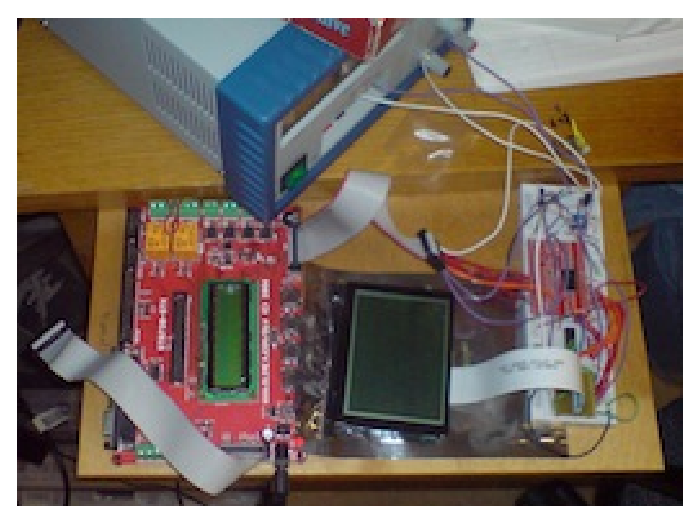
\includegraphics[width=2.5in,keepaspectratio]{results/figures/lcd_bench_test.eps}
}
\subfigure[CAN Bench test]{
  \label{fig:can_bench_test}
  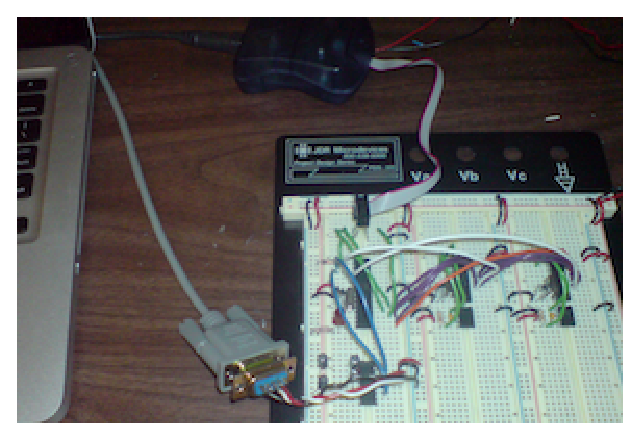
\includegraphics[width=2.5in,keepaspectratio]{results/figures/can_bench_test.eps}
}
\caption{Photographs of the driver control module bench-test experiments.}
\label{fig:bench_experiments}
\end{figure}

\subsection{Graphics Display}

Once all the hardware bugs with the driver interface module had been corrected, it was possible to continue writing the LCD interfacing software that had been started during the initial LCD testing. The external memory interface circuitry described in Sec.\ \ref{sec:lcd_module_data_interface} worked without issue. Figure \ref{fig:driver_interface_lcd} shows the LCD displaying a sample bitmap from the manufacturer.

\begin{figure}[H]
 \centering
 \includegraphics[width=5in,keepaspectratio]{results/figures/driver_interface_lcd.eps}
 \caption{Photograph of the LCD under test.}
 \label{fig:driver_interface_lcd}
\end{figure}

\subsection{Vehicle Dynamic Adjustment}

A menu system for adjusting the vehicle dynamic parameters was implemented. Turning the \emph{param} knob on the driver interface module scrolls through the list of parameters. Figure \ref{fig:driver_interface_menu} shows the LCD module displaying the parameter menu. Also visible is the system time, drawn at the top centre, the telemetry module signal strength indicator in the top right. All text in Fig.\ \ref{fig:driver_interface_menu} is drawn using the custom 16x16 font described in Sec.\ \ref{sec:lcd_module_font_loading}.

\begin{figure}[h!]
 \centering
 \includegraphics[width=3in,keepaspectratio]{results/figures/driver_interface_menu.eps}
 \caption{Photograph of the driver interface module displaying the parameter menu.}
 \label{fig:driver_interface_menu}
\end{figure}



\section{Implementation Issues Encountered}

Several specific implementation issues caused a lot of headache and project delays. All of the issues we encountered were subsequently solved.

\subsection{CAN Transceiver Hardware Bug}

After the first module, the engine and transmission module, was populated, we proceeded to inspect all solder joints and check for shorts between VCC and ground. Initially no problems were apparent, but when we first applied power to the module, using a current limiting bench power supply, a dynamic short circuit quickly appeared. The power supply immediately began limiting current, and the voltage dropped.

After a lot of searching, inspecting all the components under a microscope, and hot air rework, it was determined that the problem was not with any of the solder joints or the PCB, but in fact a problem with the schematic. In error, the circuit design for the CAN Transceiver had got the VCC and GND lines to the chip swapped. Additionally, this CAN Transceiver schematic block had been duplicated to all four modules, which resulted in the same fate.

A fix was quickly implemented, first on the engine and transmission module, and subsequently for the other modules. The copper traces to the VCC and GND pins on the CAN Transceiver were cut with an exacto knife, and rewired correctly with wire-wrap wire.

\subsection{Driver Interface LCD Reset Line}

After populating the driver interface module, an issue persisted with the active low reset line that prevented the LCD Module from being pulled out of reset with the rest of the system. Upon probing the reset line on the LCD with an oscilliscope, it was found to be oscillating at \unit{60}{\mega\hertz}. Because the LCD module uses \unit{+3.3}{\volt} logic, reset line was isolated from the rest of the system with a direction-sensing level shifter. It is hypothesized that some circuitry on the LCD module was attempting to drive the reset line, and this was causing the oscillations. Adding a very strong (\unit{120}{\ohm}) pull-up resistor to the LCD module's reset line solved the issue.

\subsection{CAN Driver Problems}

\subsection{Telemetry Module Software Race Conditions}

Multiple race conditions were caused by the large degree of asynchronous behaviour in the system, the large number of common resources used, and the multiple producer/consumer layers. These issues appeared in code that had been in use for a while on other modules, but only caused problems on the Telemetry Module. The majority of these were solved by ensuring that atomic sections were placed around critical code.

\subsection{Telemetry Module Interrupt Starvation}

Although initial average data throughput rates for both the DAC and the ECU were measured as part of the research done at the beginning of the project, non-trivial buffering issues did arise in the implementation of the telemetry module software. After several weeks of work spent debugging throughput problems with the module software, and with the aide of a protocol analyser, the root of the problem was tracked down. The AT90CAN microcontroller's interrupt vectors are fixed at the factory, therefore the priority of interrupts on the microcontroller is fixed. Unfortunately this lead to a resource starvation issue. The MAX3100 UART uses an external interrupt line, which has priority over the internal UART interrupts. When there is data in the MAX3100's transmit buffer, the MAX3100's interrupt handler will starve the internal UART interrupt to a certain extent. This was investigated by saturating the MAX3100 output buffer with a constant stream of data, and then inputting some bytes to the internal UART. Single input bytes were read properly, but any long stream of incoming bytes (more than 4 in a row) would cause hardware input buffer overruns in the built-in UART, and incoming data would be lost.

\begin{figure}[ht]
  \centering
  \label{fig:ecu_data}
  \begin{tikztimingtable} %[timing/nice tabs]
    $ECU_{Rx}$ & Z 10D{Polling sequence (7 bytes)} 14F Z \\
    $ECU_{Tx}$ & 12Z 6D{Reply sequence} ;[dotted] 2D{...}; 5D{(539 bytes)} Z\\
    \extracode
      %\tableheader{Signal}{Timing}
      \tablerules
  \end{tikztimingtable}
  \caption{ECU Serial Data Example}
  \label{fig:ecu_serial_data}
\end{figure}

Based on this knowledge, we were able to classify conditions where the software would be unable to accurately process the incoming data. Unfortunately the method that the ECU transmits it's data falls within this characterization. When the ECU is communicating with the DTASWin software, the software will send a handful of bytes (around 7) to the ECU, and the ECU will respond with one large packet of approximately 540 bytes, as shown in Fig.\ \ref{fig:ecu_serial_data}. If the MAX3100 is transmitting a large amount of data when this large packet comes in, bytes will be lost from the interrupt starvation issue.

Having determined the problem, several options lay before us to resolve the issue:
\begin{itemize}
  \item By lumping the ISR handlers for both the internal UART and the MAX3100 together, it would be possible to conditionally alter the priority of the processing to allow the incoming data to take precedence. This would however override the natural encapsulation that the two drivers had, and would require writing specialized drivers for use only on the telemetry module;
  \item Throttling the transmission of data to the MAX3100 by sequenced enabling and disabling of the interrupt could also reduce the starvation issue, but getting the sequencing and timing right would be difficult and more than likely result in further problems;
  \item Finally, the method successfully used in the implementation was to enabled nested interrupts from the MAX3100 interrupt handler. This is done in two steps at the beginning of the interrupt handler:
  \begin{itemize}
   \item First, the MAX3100 external interrupt is disabled, to prevent it recursively firing;
    \item then, global interrupts are re-enabled. This allows the UART to interrupt the MAX3100 interrupt when it receives a byte.
  \end{itemize}
\end{itemize}